\documentclass[12pt]{ociamthesis}  % default square logo 
%\documentclass[12pt,beltcrest]{ociamthesis} % use old belt crest logo
%\documentclass[12pt,shieldcrest]{ociamthesis} % use older shield crest logo

%load any additional packages
\usepackage{amssymb}

%input macros (i.e. write your own macros file called mymacros.tex 
%and uncomment the next line)
%\include{mymacros}

\title{Panduan Tingkat Akhir\\[1ex]     %your thesis title,
        Tugas Akhir}   %note \\[1ex] is a line break in the title

\author{ Syafrial Fachrie Pane}             %your name
\college{Kordinator Tugas Akhir}  %your college

%\renewcommand{\submittedtext}{change the default text here if needed}
\degree{Politeknik Pos Indonesia}     %the degree
\degreedate{Bandung 2019}         %the degree date

%end the preamble and start the document
\begin{document}

%this baselineskip gives sufficient line spacing for an examiner to easily
%markup the thesis with comments
\baselineskip=18pt plus1pt

%set the number of sectioning levels that get number and appear in the contents
\setcounter{secnumdepth}{3}
\setcounter{tocdepth}{3}


\maketitle                  % create a title page from the preamble info
\begin{dedication}
This thesis is dedicated to\\
 someone\\
for some special reason\\
\end{dedication}        % include a dedication.tex file
\begin{acknowledgements}
plenty of waffle, plenty of waffle, plenty of waffle, plenty of waffle,
plenty of waffle, plenty of waffle, plenty of waffle, plenty of waffle.
\end{acknowledgements}   % include an acknowledgements.tex file
\begin{abstract}
	Buku Pedoman ini dibuat dengan tujuan memberikan acuan, bagi mahasiswa Tingkat Akhir dan dosen
	Pembimbing. Pada intinya buku ini menjelaskan secara lengkap tentang Standar pengerjaan Intership  dan 
	Tugas Akhir
	di Program Studi D4 Teknik Informatika, dan juga mengatur mekanisme, teknik penulisan, serta
	penilaiannya.Dengan demikian diharapkan semua pihak yang terlibat dalam aktivitas Bimbingan Mahasiswa Tingkat Akhir
	berjalan lancar dan sesuai dengan standar.
\end{abstract}          % include the abstract

\begin{romanpages}          % start roman page numbering
\tableofcontents            % generate and include a table of contents
\listoffigures              % generate and include a list of figures
\end{romanpages}            % end roman page numbering

%now include the files of latex for each of the chapters etc
\chapter{Standar Pengajuan}

Pada pengajuan kali ini. Setiap mahasiswa tingkat akhir wajib untuk menemui pembimbing untuk menyepakati judul, metode, sumber data, abstrack dan referensi yang akan digunakan dalam penelitian. Sebelum pertemuan dengan pembimbing, mahasiswa wajib sudah membuat resume dari 15 jurnal dalam 5 tahun terakhir yang terindex scopus(cek di scimagojr.com) dan dituangkan di template presentasi. Template presentasi terdapat di situs informatika. Mahasiswa wajib melakukan presentasi terlebih dahulu ke pembimbing dengan template presentasi kemudian baru melakukan diskusi.Pengajuan penelitian tingkat akhir yaitu Tugas Akhir dilakukan melalui formulir online yang diberikan dan diisi bersama dengan Pembimbing apabila sudah disepakati dan disetujui bersama pembimbing. Pengisian form menggunakan email poltekpos dari pembimbing. Pastikan sudah melakukan login dengan email poltekpos terlebih dahulu oleh pembimbing. Formulir bisa diakses pada laman situs if.poltekpos.ac.id. Perlu diperhatikan Formulir yang perlu diisi terdiri dari :
\begin{enumerate}
\item Judul yang diajukan dalam bahasa inggris
\item abstrack berbahasa inggris terdiri dari 150-250 kata.
\item ringkasan yang terdiri dari metode yang digunakan, Data Penilitian (sumber data yang digunakan dan jumlah data yang digunakan)
\item daftar referensi
\end{enumerate}
Dari point diatas perlu diperhatikan adalah standar pengisian form masing-masing. Pembimbing Utama Tugas Akhir adalah pembimbing dari Internship yang telah dipetakan dan disesuaikan syarat pembimbing yaitu memiliki pangkat akademik minimal asisten ahli jika tidak terpenuhi maka dosen pembimbing tersebut akan dipetakan sebagai pembimbing pendamping. Setiap mahasiswa tingkat akhir harus memperhatikan data dosen yang terdapat pada situs Informatika pada menu tim seperti terlihat pada gambar \ref{figure:timif}.
\begin{figure}[ht]
	\centerline{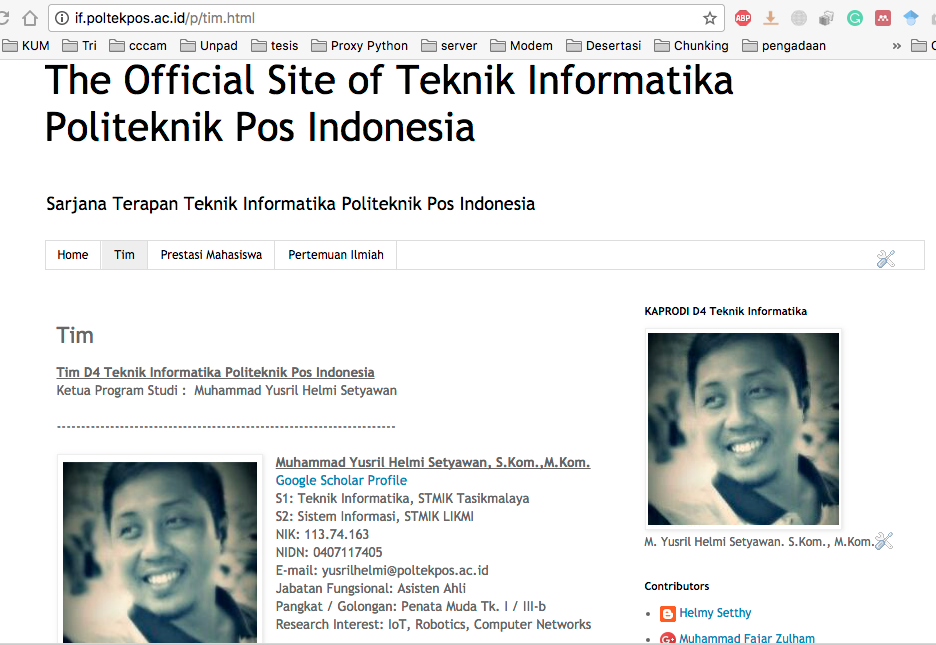
\includegraphics[width=0.5\textwidth]{figures/timif.png}}
	\caption{Data Pembimbing dari situs informatika.}
	\label{figure:timif}
	\end{figure}
Setiap mahasiswa wajib mematuhi aturan dari masing-masing pembimbing tentang tata cara komunikasi dan aturan bimbingan yang bisa diakses dari laman portal dosen masing-masing yang terdapat pada situs informatika atau pertemuan langsung dengan pembimbing. Standar pengisian form pengajuan judul penelitian harus sesuai dengan standar pengajuan pada chapter ini. berikut proses pengajuan judul tugas akhir pada gambar \ref{figure:P1}.
\begin{figure}[ht]
	\centerline{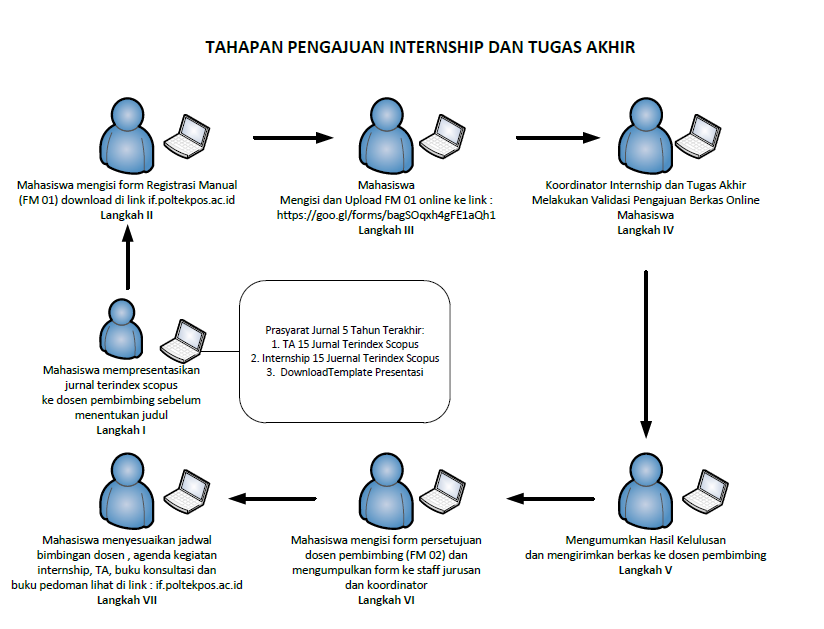
\includegraphics[width=1\textwidth]{figures/pengajuan.png}}
	\caption{Tahapan Pengajuan Judul Internship dan Tugas Akhir.}
	\label{figure:P1}
	\end{figure}
Penjelasan pada gambar  \ref{figure:P1} mahasiswa setelah bertemu dengan dosen pembimbing maka mengisi form 01 yang terdiri dari Judul dan Abstract.
\section{Judul}
Judul menggunakan bahasa Inggris. Judul diutamakan dapat menggambarkan riset dan metode yang akan dilakukan. Pemilihan judul juga harus dengan kesepakatan pembimbing. 

\section{Abstract}
Abstrak mengunakan bahasa inggris aktif dan positif. Tidak terdapat sitasi pada abstrak. Kalimat harus utuh terdiri dari Subjek Predikat Objek dan boleh ditambahkan Keterangan. Tidak boleh menggunakan kalimat pasif atau kalimat negatif. Abstrak harus terdiri dari 150-250 kata. Abstrak berisi latar belakang, tujuan, metode, dan target output dari penelitian.

\section{Ringkasan}
\subsection{Metode}
Metode yang digunakan adalah metode yang terdapat pada referensi dalam 5 tahun terakhir dari jurnal internasional terindex scopus. Penelitian harus menggunakan atau mengkombinasikan minimal 2 metode yang berbeda.

\subsection{Data Penelitian}
Sumber data penelitian harus ditargetkan dan jelas dari mana sumbernya. Sebutkan dari mana sumber datanya, berapa banyak datanya serta diskusikan bersama pembimbing mengenai jenis data apa saja yang harus didapatkan. 

\section{Referensi}
Semua referensi yang digunakan harus terindex pada google scholar. Minimal 15 referensi dari jurnal terindeks Scopus dan merupakan artikel dalam 5 tahun terakhir. Jurnal yang terindex scopus bisa dicek di situs scimagojr.com. Format referensi yang disikan pada formulir pengajuan penelitian tingkat akhir adalah BibTex. BibTex referensi bisa didapatkan pada laman Google Scholar. selain jurnal referensi dalam kutipan bisa bersumber dari berita atau undang - undang yang bekaitan dengan penelitian yang diajukan/dikerjakan.




\chapter{Standar Penulisan Jurnal}

Penulisan jurnal harus menggunakan Latex dengan template IEEE. Template bisa di unduh pada menu dokumen portal kampus keren atau situs informatika. Penulisan jurnal harus mengikuti standar penulisan akademis dan mengikuti kerangka jurnal. Jurnal wajib menggunakan bahasa inggris(Amerika) yang dikoreksi bersama pembimbing atau kolaborator. 

\section{Standar Penulisan}
Di dalam penulisan artikel ilmiah harus mengikuti standar minimal penulisan ilmiah. Standar ini digunakan untuk menyamakan semantik bahasa agar tulisan lebih mudah dibaca dan dipahami. Penggunaan standar merupakan keniscayaan dalam penulisan artikel ilmiah.
\subsection{Penggunaan Kalimat}
Penulisan jurnal harus menggunakan kalimat aktif dan positif. Memiliki Subject, Predikat dan Object yang jelas. Tidak bertele-tele dan terlalu panjang dalam penggunaan kalimat(terlalu banyak kata sambung dan tanda koma). Satu paragraf minimal terdiri dari tiga kalimat. Hindari paragraph yang terdiri dari satu kalimat yang biasanya digunakan untuk penjelasan gambar, rumus atau tabel. Lebih baik digabungkan saja dengan narasi paragraph sebelumnya. Jika memang harus ada penjelasan kalimat, maka kembangkan lagi menjadi narasi satu paragraph utuh. Tidak boleh menulis kata ganti orang seperi Penulis, Saya, Kami, Mereka. Gunakan kata benda seperti penelitian ini, riset ini.

\subsection{Penempatan Sitasi}
Sitasi ditempatkan tepat pada akhir kalimat penjelasan referensi sebelum tanda 
pemisah antar kalimat (koma atau titik) tanpa spasi. 
Sitasi juta dapat ditumpuk pada sebuah kalimat yang merupaka  penjelasan singkat dari referensi. 
Please ensure that: all references have been cited in your text. Each citation should be written in the order of appearance in the text. The references must be presented in numbering. 

\subsection{gambar, rumus, tabel}
Pemanfaatan instrumen pendukung gambar kualitasnya harus ditingkatkan, jangan sampai terdapat gambar yang tidak bisa terbaca tulisannya.
Tidak diperbolehkan memberikan narasi penunjukan relatif. seperti :
\begin{itemize}
	\item Lebih detailnya lihat gambar di bawah ini
	\item Untuk lebih jelasnya lihar rumus di bawah ini
	\item data bisa dilihat di tabel di atas
\end{itemize}
Diperbaiki yang seharusnya :
\begin{itemize}
	\item Pada gambar 1.1 terlihat bahwa hasil perhitungan penduduk sudah mulai jenuh.
	\item Total kejenuhan hasil kalkulasi terlihat di tabel 1.1.
	\item Rumus 1.1 merupakan rumus kalkulasi tingkat kejenuhan.
\end{itemize}
Prepare your figures in high quality and created by yourself (not copy and paste from other parties). All legends, captions, etc in your figures MUST in English.


\section{Kerangka Jurnal}
Kerangka acuan dalam membuat jurnal harus memenuhi standar acuan di sub bab ini. Masing-masing kerangka jurnal harus memenuhi standar dan aturan yang ditetapkan. Pengerjaan jurnal biasanya lebih awal daripada pengerjaan laporan.Bagian-bagian dari jurnal terdiri dari abstrak (Abstract), pendahuluan (Introduction), metode (Methods), Penelitian Terkait (Related Works),percobaan (Experiment), hasil (Result) dan diskusi (Discussion).

\subsection{Judul}
Maksimal 10 (sepuluh) kata dalam Bahasa Inggris ringkas dan tegas.

\subsection{Abstract}
Terdiri dari 150-200 kata tanpa ada sitasi. Berisi latar belakang, tujuan,metode, hasil,kesimpulan dan saran. Pada abstrak harus dimunculkan persoalan utama dan pentingnya melakukan penelitian ini, serta solusi yang diusulkan. Isi tertuang dengan kalimat yang jelas.Kata kunci atau keyword ditentukan dengan nama metode yang digunakan dan sub sub bidang penelitian yang dilakukan. Kata kunci minimal harus terdapat lima kata kunci.

\subsection{Introduction}
Pada bagian pendahuluan uraikan rincian persoalan terkini berdasarkan beberapa referensi dari jurnal intenasional yang di sitasi, sehingga penelitian ini layak dilakukan. An Introduction should contain the following three parts:
\begin{itemize}
    \item Background: Authors have to make clear what the context is. Ideally, authors should give an idea of the state-of-the art of the field the report is about.
    \item  The Problem: If there was no problem, there would be no reason for writing a manuscript, and definitely no reason for reading it. So, please tell readers why they should proceed reading. Experience shows that for this part a few lines are often sufficient.
    \item The Proposed Solution: Now and only now! - authors may outline the contribution of the manuscript. Here authors have to make sure readers point out what are the novel aspects of authors work.
\end{itemize}
Authors should place the paper in proper context by citing relevant papers. Setiap ada pemaparan data, informasi, dan sebuah pernyataan pada sebuah kalimat maka wajib diakhiri dengan sitasi.Minimal terdapat sitasi pada setiap kalimat pernyataan, informasi, dan data pada bagian Introduction dari jurnal 5 tahun terakhir terindex scopus.

\subsection{Related Works}
Penjelasan singkat dengan sitasi dari artikel yang direferensikan minimal dari 10 artikel. Artikel yang dijelaskan merupakan artikel yang terkait dengan kata kunci penelitian. Minimal 3 Paragraph. Pada paragraph terakhir harus ada pernyataan perbedaan antara penelitian yang akan dilakukan dengan penelitian yang disebutkan pada sitasi di related works.

\subsection{Method}
Penjelasan teknis yang jelas dan gamblang mengenai metode yang digunakan dengan sitasi. Terdiri dari definisi, konsep, rumus atau diagram. Metode yang digunakan adalah metode yang terdapat pada referensi dalam 5 tahun terakhir  dari  jurnal  internasional  terindex  scopus. 

\subsection{Experiment}
Data sumber yang jelas dan cukup untuk dijadikan penelitian, disertai dengan hasil nya sesuai langkah-langkah yang di tuliskan di Method.

\subsection{Result and Discussion}
Sangat jelas relevasinya dengan latar belakang dan pembahasan, dirumuskan dengan singkat. The presentation of results should be simple and straightforward in style. You should improve your analyzing and also present the comparison between performance of your approach and other researches. Results given in figures should not be repeated in tables. This section report the most important findings, including results of analyses as appropriate. It is very important to prove that your manuscript has a significant value and not trivial.

\subsection{Reference}
Semua  referensi  yang  digunakan  harus  terindex  pada  google  scholar.   Minimal  15 referensi dari jurnal terindeks Scopus dan merupakan artikel dalam 5 tahun terakhir. Jurnal yang terindex scopus bisa dicek di situs scimagojr.com.  Format referensi yang disikan  pada  formulir  pengajuan  penelitian  tingkat  akhir  adalah  BibTex.   BibTex referensi bisa didapatkan pada laman Google Scholar.

\section{Standar Format Latex}
Beberapa Aturan yang harus dipatuhi :
\begin{enumerate}

    \item file disimpan dalam format ber ekstensi .tex per chapter masing2 di folder section

    \item gambar disimpan dalam folder figures dengan namagambar

    \item referensi dari google scholar,scholar.google.com

    \item Setiap referensi yang diambil, maka tambahkan dan tuliskan ke dalam file bernama references.bib yang berisi kumpulan bibTex dari referensi. Gunakan standar pengutipan yang baik dan benar

    \item Gambar disebutkan di dalam artikel dengan format sesuai labelnya yaitu \\ \verb|\ref{labelgambar}|. \\ Gambar diselipkan dengan menambahkan blok sintaks :
    \begin{verbatim}
    \begin{figure}[ht]
    \centerline{\includegraphics[width=1\textwidth]
    {figures/namagambar.JPG}}
    \caption{penjelasan keterangan gambar.}
    \label{labelgambar}
    \end{figure}
    
    Contoh :
    Pada gambar \ref{labelgambar} dijelaskan bahwa 
    sistem operasi memiliki 3 versi.
    \end{verbatim}

    \item Referensi disebutkan dengan menyebutkan nama di dalam file bibtex No.4. \\
    Contoh, Jika Bibtex sudah diinputkan kedalam reference.bib seperti ini :
    \begin{verbatim}
    @inproceedings{ganapathi2006windows,
      title={Windows XP Kernel Crash Analysis.},
      author={Ganapathi, Archana and Ganapathi, 
      Viji and Patterson, David A},
      booktitle={LISA},
      volume={6},
      pages={49--159},
      year={2006}
    }
    \end{verbatim}
    Maka penulisan kalimat di jurnal : \\
    Dalam sebuah artikel dari Ganapathi yang 
    menyebutkan bahwa komputasi adalah keniscayan \verb|\cite{ganapathi2006windows}|.
    
    \item Penyebutan subbab dan subsubbab diatur dengan cara : \\
    judul sub bab : \\ 
    \verb|\section{nama sub bab}| \\
    judul sub sub bab ditulis dengan :\\ 
    \verb|\subsection{judul sub sub bab} | \\
    judul sub sub sub bab ditulis dengan : \\ \verb|\subsubsection{Judul sub sub sub bab} | \\
    contoh :
    \begin{verbatim}
    \section{Sejarah Peta}
Perkembangan peta dunia tidak luput dari para ahli 
geografi dan kartografi. Peta dunia yang populer pada saat 
ini merupakan 
kontribusi dari para 
pembuat peta sebelumnya

\subsection{Ptolemy's}
Ptolemy's diduga membuat peta pada abad ke 2
\end{verbatim}
    
    \item untuk list dan nomor gunakan enumerate atau itemize contoh :
    \begin{verbatim}
berikut nama anggota kelompok
\begin{enumerate}
\item darso
\item karyo
\item doyok
\end{enumerate}

\begin{enumerate}
\item
This is the first item in the numbered list.

\item
This is the second item in the numbered list.
\end{enumerate}

\begin{itemize}
\item
This is the first item in the itemized list.

\item
This is the first item in the itemized list.
This is the first item in the itemized list.
This is the first item in the itemized list.
\end{itemize}

\begin{itemize}
\item[]
This is the first item in the itemized list.

\item[]
This is the first item in the itemized list.
This is the first item in the itemized list.
This is the first item in the itemized list.
\end{itemize}
    \end{verbatim}
    
    \item spesial karakter menggunakan tanda `\verb|\|' didepannya contoh :
    \begin{verbatim}
\& 
\% 
\$ 
\#  
\{ \}
\_
\"dalam petik\"
`dalam petik'
jika spesial karakter menjadi banyak atau satu baris gunakan verb
contoh :
\verb|%$'%&$&'%'%'%&'%|
    \end{verbatim}
    
    \item untuk tabel gunakan table , dan jangan lupa tabel di referensikan pada kalimat berdasarkan labelnya. contoh:
    \begin{verbatim}
ini merupakan contoh tabel \ref{table:contoh} ukuran kecil.
\begin{table}[h]
\caption{Small Table}
\centering
\begin{tabular}{ccc}
\hline
one&two&three\\
\hline
C&D&E\\
\hline
\end{tabular}
\label{table:contoh}
\end{table}
    \end{verbatim}
    
    \item untuk rumus gunakan tag equation dan di referensikan pada kalimat dengan tag ref sesuai labelnya contoh:
    \begin{verbatim}
Luas permukaan dijelaskan pada rumus \ref{eq:1}.Volume dijelaskan 
pada rumus \ref{eq:2}.
$L$ merupakan luas, $\pi$ adalah 3,14.
\begin{equation}\label{eq:1}
     L = 4 \pi r^2 \,
\end{equation}
 \begin{equation}\label{eq:2}
     V = \frac{4}{3}\pi r^3
\end{equation}
    \end{verbatim}
    
    \item untuk kode program menggunakan verbatim
    \begin{verbatim}
\ begin{verbatim}
a = "anu"
b = "itu"
c = a + b
print(c) 
\ end{verbatim}
    \end{verbatim}
\end{enumerate}





\chapter{Standar Penulisan Laporan}

Penulisan Laporan untuk internship dan Tugas Akhir . 

\section{Kerangka Penulisan}
Penulisan laporan internship dan tugas akhir harus mengikuti kerangka yang telah di tentukan sebagai berikut :

\begin{enumerate}
\item
Bagian Awal terdiri dari :
\begin{enumerate}
\item lembar muka/cover halam depan bahasa indonesia dan bahasa inggris ; (hal. Lampiran)
\item lembar pengesahan dari perusahaan dan prodi/jurusan; (hal. Lampiran) 
\item surat pernyataan tidak melakukan plagiarisme ; (hal. Lampiran)
\item abstrak (dalam Bahasa Indonesia); (hal. Lampiran)
\item abstract (dalam Bahasa Inggris); (hal. Lampiran)
\item kata pengantar; (hal. Lampiran)
\end{enumerate}
Daftar isi termasuk :
\begin{enumerate}
\item lembar muka/cover halam depan bahasa indonesia dan bahasa inggris ; (hal. Lampiran)
\item lembar pengesahan dari perusahaan dan prodi/jurusan; (hal. Lampiran) 
\item	daftar gambar; (hal. Lampiran)
\item	daftar tabel; (hal. Lampiran)
\item	daftar simbol; (hal. Lampiran)
\item	daftar singkatan; (hal. Lampiran)
\item	daftar lampiran. (hal. Lampiran) 

\end{enumerate}
\item
Bagian Isi terdiri dari :
\begin{enumerate}
\item BAB I Pendahuluan
\begin{itemize}
\item 1.1.	Latar Belakang 
\item 1.2.	Identifikasi Masalah 
\item 1.3.	Tujuan dan Manfaat 
\item 1.4.	Ruang Lingkup 
\item 1.5.	Penelitian Sebelumnya
\item 1.6.	Gambaran Umum Metodologi Penelitian 
\end{itemize}
\item BAB II Landasan Teori
\item BAB III Gambaran Organisasi Perusahaan
\begin{itemize}
\item 3.1.	Sejarah Perusahaan
\item 3.2.	Visi dan Misi Perusahaan
\item 3.3.	Struktur Organisasi dan Job Description Perusahaan 
\item 3.4.	Deskripsi dan Ruang Lingkup Internsip/Tugas Akhir
\end{itemize}
\item BAB IV Metodologi Penelitian
\begin{itemize}
\item 4.1.	Diagram Alur Metodologi Penelitian.
\item 4.2.  Tahapan – Tahapan Diagram Metodologi Penelitian

Untuk menentukan diagram alur Metodologi Penelitain bisa menggunakan jurnal terindex scopus.
 
\end{itemize}
\item BAB V Analisis dan Sistem
\begin{itemize}
\item 5.1.	Analisis sistem yang berjalan
\item 5.2.	Analisis sistem yang akan dibangun
\item 5.3.	Analisis dan Perancangan Database
\item 5.4.	Analisis dan Perancangan User Interface Sistem. 
\item 5.5.	Analisis dan Perancangan Arsitektur Sistem/Aplikasi.
\end{itemize}
\item BAB V Pembahasan dan Evaluasi


Pembahasa yang dilakukan dengan cara mengukur dari hasil analisi dengan menggunakan framwork dan metode yang ada.
\item BAB VI Penutup
\begin{itemize}
\item 6.1.	Kesimpulan
\item 6.2.  Saran

merangkum dan menjawab dari hasil keseluruhan masalah yang ada
 
\end{itemize}
\item Daftar Pustaka

Ketentuan dalam penulis kajian pustaka menggunakan format IEEE dan referensi yang bersumber dari jurnal terindex scopus terdiri dari
\begin{itemize}
\item
Internship dan Tugas Akhir : 15 jurnal terindex scopus dan 5 referensi perpustakaan Politeknik Pos Indonesia
\end{itemize}
\item Lampiran
\end{enumerate}
\end{enumerate}

\section{Ukuran Kertas, Jenis Kertas dan Huruf}
Penulisan laporan internship dan tugas akhir harus mengikuti ukuran kertas, jenis kertas dan huruf sebagai berikut :
\begin{enumerate}
\item Ukuran kertas adalah A4 (2 x 29,7 Cm), dengan berat kertas 80 gram
\item Judul bab diketik dengan menggunakan huruf besar (kapital), font Arial, 16 point, Bold, dan diletakkan ditengah-tengah (center); sedangkan sub bab menggunakan 14 point. Jarak antara isi tesis dengan sub bab adalah 4 spasi, dan pengetikan angka pada judul tiap bab memakai angka Romawi. Isi laporan diketik dengan menggunakan font Times New Roman, 12 point, 2 spasi.. Penulisan dan ejaan menggunakan ketentuan bahasa Indonesia yang baik dan benar (EYD). penulisan dengan ketentuan : \begin{enumerate}
\item Batas pengetikan 4 cm dari pinggir kertas sebelah kiri
\item 3 cm dari pinggir kertas sebelah atas, bawah, dan kanan
This is the secon
\item Nomor halaman ditempatkan pada sebelah kanan atas dengan angka Arab (1, 2, 3, …), kecuali pada halaman judul bab nomor halaman diletakkan di tengah (center) bagian bawah, yang mencakup (termasuk) daftar acuan, daftar pustaka, dan semua lampiran (sampai halaman paling akhir).
\item Khusus pada nomor halaman sebelum Bab I, yaitu mulai dari halaman sampul sampai dengan Daftar Isi/Tabel menggunakan angka Romawi ( i, ii, iii, iv, …) yang diletakkan di tengah bagian bawah. Pada halaman judul bab, nomor halaman juga diletakkan di tengah bagian bawah.
\item Judul tabel ditulis dengan jarak satu spasi di atas tabel. Untuk huruf pertama setiap kata ditulis huruf besar (kecuali kata sambung di, pada, ke, dengan, dan sebagainya). Judul gambar / grafik / bagan diletakkan di bawah gambar dengan ketentuan penulisan seperti judul tabel. Judul diberi nomor urut dengan angka biasa.
\item Kutipan tulisan di tulis dengan standart IEEE.
\item Laporan ditulis dalam bahasa Indonesia, laporan yang berbahasa Indonesia harus mengikuti ketentuan Ejaan yang Disempurnakan (EYD) 1975 dan Pedoman Umum Pembentukan Istilah (PUPI), termasuk tata cara penggunaan tanda baca dan pemutusan kata, serta tidak menggunakan kata asing untuk kata yang sudah mempunyai padanan kata dalam bahasa Indonesia. Kata asing harus ditulis Italic. Singkatan harus ditulis secara lengkap ketika pertama kali digunakan dengan singkatannya dalam tanda kurung, seterusnya cukup menggunakan singkatannya saja.
\end{enumerate}
\section{Acuan/Daftar Pustaka/Kajian Pustaka}
Ketentuan dalam penulis kajian pustaka menggunakan format IEEE dan referensi yang bersumber dari jurnal terindex scopus terdiri dari
\begin{itemize}
\item
Internship dan Tugas Akhir : 15 jurnal terindex scopus dan 5 referensi perpustakaan Politeknik Pos Indonesia

\item
The template will number citations consecutively within brackets [1]. The sentence punctuation follows the bracket [2]. Refer simply to the reference number, as in [3]—do not use “Ref. [3]” or “reference [3]” except at the beginning of a sentence: “Reference [3] was the first ...”
Number footnotes separately in superscripts. Place the actual footnote at the bottom of the column in which it was cited. Do not put footnotes in the reference list. Use letters for table footnotes.
Unless there are six authors or more give all authors’ names; do not use “et al.”. Papers that have not been published, even if they have been submitted for publication, should be cited as “unpublished” [4]. Papers that have been accepted for publication should be cited as “in press” [5]. Capitalize only the first word in a paper title, except for proper nouns and element symbols.
For papers published in translation journals, please give the English citation first, followed by the original foreign-language citation [6].

\end{itemize}
\end{enumerate}

 
\chapter{Kelengkapan Internship dan Tugas Akhir}

\section{Tahapan Pergantian Judul}
Lhat pada gambar \ref{figure:P2}.
\begin{figure}[ht]
	\centerline{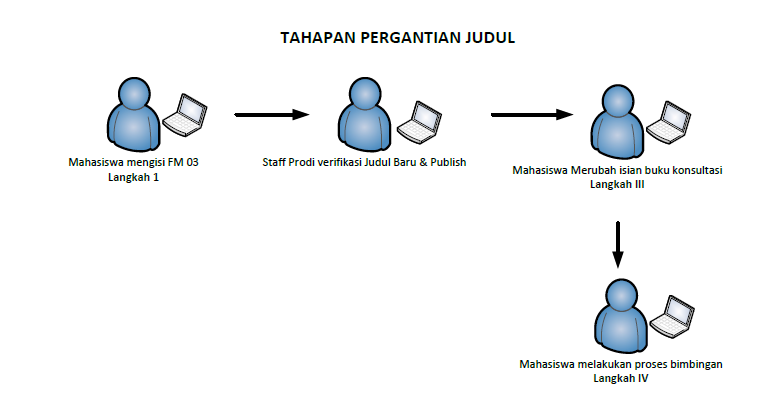
\includegraphics[width=1\textwidth]{figures/ganti_judul.png}}
	\caption{Tahapan Pergantian Judul}
	\label{figure:P2}
	\end{figure}

\section{Tahapan Pengajuan Sidang}
Lhat pada gambar \ref{figure:P3}.
\begin{figure}[ht]
	\centerline{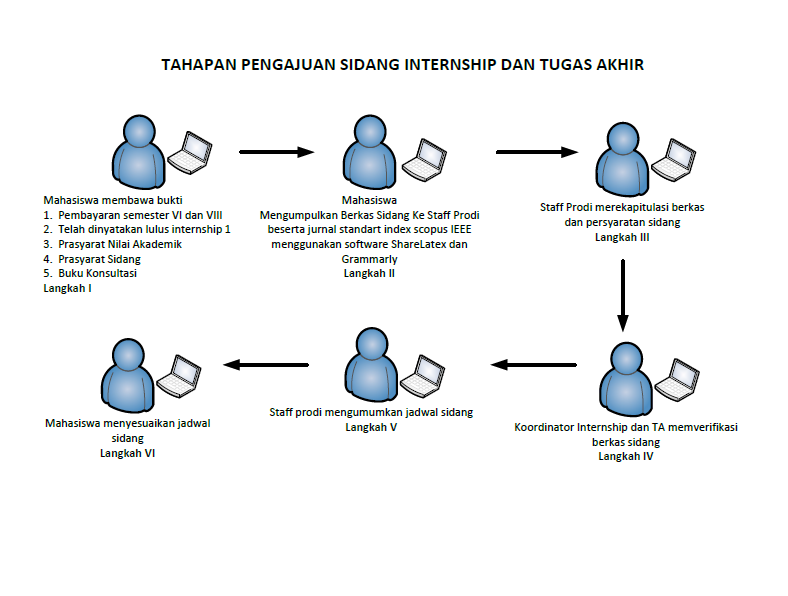
\includegraphics[width=1\textwidth]{figures/draft.png}}
	\caption{Tahapan Pengajuan Sidang}
	\label{figure:P3}
	\end{figure}
\section{Tahapan Revisi Laporan dan Jurnal}
Lhat pada gambar \ref{figure:P31}.
\begin{figure}[ht]
	\centerline{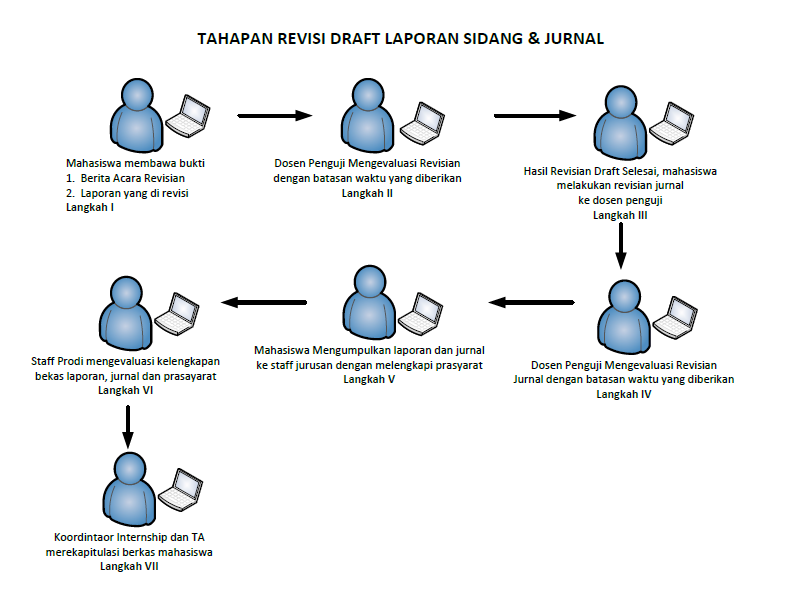
\includegraphics[width=1\textwidth]{figures/revisi.png}}
	\caption{Tahapan Revisi Laporan dan Jurnal}
	\label{figure:P31}
	\end{figure}
\section{Tahapan Sidang Ulang}
Lhat pada gambar \ref{figure:P4}.
\begin{figure}[ht]
	\centerline{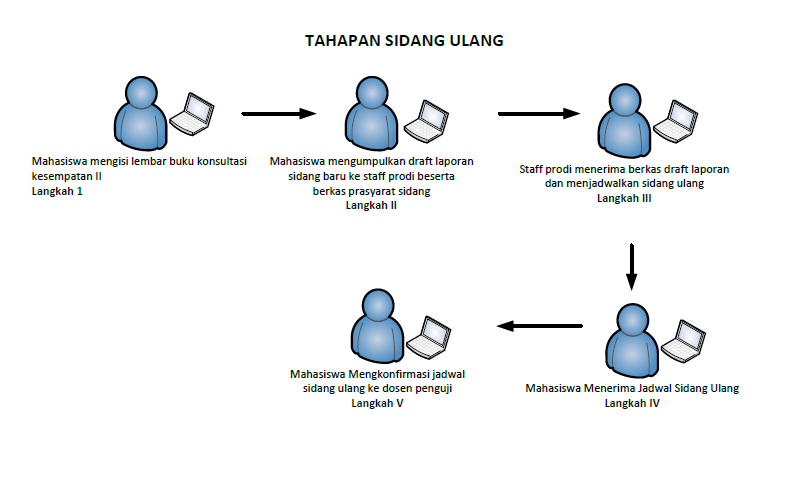
\includegraphics[width=1\textwidth]{figures/ulang.png}}
	\caption{Tahapan Sidang Ulang}
	\label{figure:P4}
	\end{figure}
\section{Tahapan Sidang Kode Etik}
Lhat pada gambar \ref{figure:P5}.
\begin{figure}[ht]
	\centerline{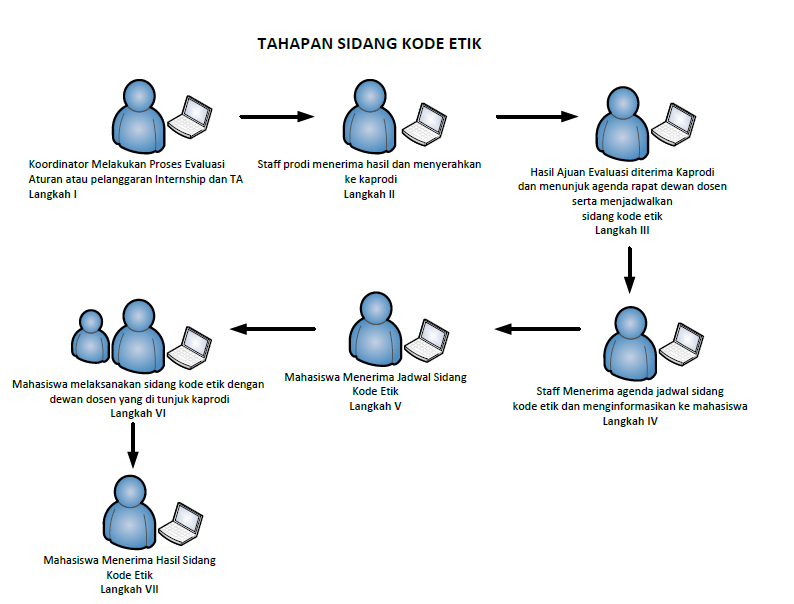
\includegraphics[width=1\textwidth]{figures/kode.png}}
	\caption{Tahapan Sidang Kode Etik}
	\label{figure:P5}
	\end{figure}
	
	
\chapter{Pengajuan Sidang dan Publikasi}

\section{Sidang dan Publikasi Tugas Akhir}
Pra-syarat penyelenggaran sidang dan publikasi antara lain:
\begin{enumerate}
	\item melengkapi data dan mencetak form sidang yang ada di menu Intranet portal if. Untuk yang metode publikasi, tanggal sidang diganti dengan tanggal diterimanya artikel pada jurnal tujuan. 
	\item Form sidang dimasukkan ke dalam Map Plastik Warna merah(lihat gambar \ref{mapplastik}), pada plastik bagian luar, depan di pojok kanan atas ditempel stiker label (lihat gambar \ref{label}) yang berisi nomor urut dari form penilaian tingkat akhir tab Tugas Akhir, Nama, NPM, Pembimbing I dan II yang diketik dan di print rapih pada stiker(lihat gambar \ref{labelcon}). Lampirkan juga surat diterimanya jurnal untuk diterbitkan(Jika ada).
	\item Pastikan oleh anda sendiri pembimbing sudah mengisi jadwal sidang di kolom Nilai Tingkat Akhir tab Tugas Akhir.
\end{enumerate}

\begin{figure}[ht]
	\centerline{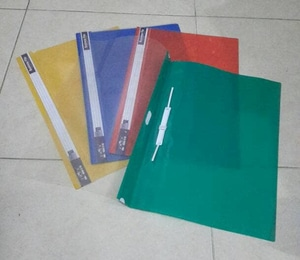
\includegraphics[width=.25\textwidth]{figures/mapplastik}}
	\caption{Map Plastik}
	\label{mapplastik}
	\end{figure}
	
	\begin{figure}[ht]
		\centerline{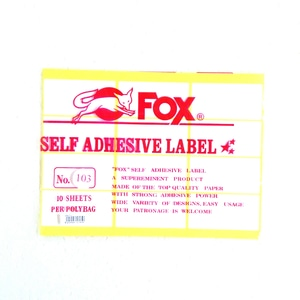
\includegraphics[width=.25\textwidth]{figures/label}}
		\caption{Stiker Label}
		\label{label}
		\end{figure}

		\begin{figure}[ht]
			\centerline{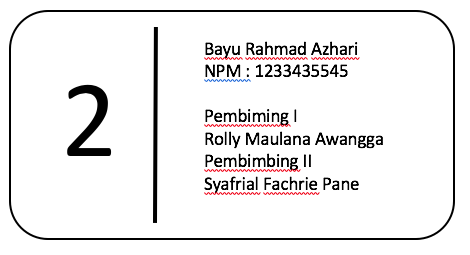
\includegraphics[width=.25\textwidth]{figures/labelcon}}
			\caption{Contoh Penulisan di Stiker}
			\label{labelcon}
			\end{figure}


Metode penilaian tugas akhir mahasiswa berhak untuk memilih dua metode, yaitu metode sidang dan publikasi.
\subsection{Metode Sidang}
Metode pertama adalah metode sidang. Metode sidang hanya diperbolehkan untuk mahasiswa dengan nilai akhir C. 
Pengajuan Jadwal Sidang TA silahkan berkordinasi dengan kedua pembimbing dan input langsung oleh pembimbingnya hari tanggal dan jamnya pada form nilai tingkat akhir tab Tugas AKhir. Pada saat sidang pastikan membawa map plastik yang sudah lengkap formnya. Membawa laporan, jurnal, dan slide PPT. Beberapa ketentuan standar pelaksanaan sidang yang wajib dipenuhi antara lain: 
\begin{enumerate}
	\item Form Pada Map sudah dilengkapi
	\item pada slide presentasi; Font ukuran minimal 24. Tidak boleh kurang dari ukuran font 24.
	\item pada slide presentasi; Paparkan referensi terlebih dahulu, kenapa memilih alasan referensi tersebut di daftar pustaka. Kemudian sebutkan target publikasi jurnalnya.
	\item Perlihatkan hasil scan plagiarisme dari laporan dan jurnal.
	\item Bawakan dan Sampaikan dalam bahasa Inggris selama sidang.
	\item Sampaikan presentasi dengan waktu kurang dari 10 menit. Pastikan anda membawa stop watch atau HP yang memiliki timer dengan settingan 10 menit.
\end{enumerate}
Selesai sidang, jika terdapat revisi maka selesaikan sebelum jangka waktu yang ditentukan. Untuk publikasi status sudah diterima maksimal sebelum jadwal UAS.

\subsection{Metode Publikasi}
Metode kelulusan dengan publikasi merupakan salah satu metode yang digunakan oleh perguruan tinggi di Australia dalam meluluskan mahasiswanya.
Dengan metode ini mahasiswa tidak diperlukan untuk melakukan sidang. Mahasiswa cukup mempublikasikan hasil karya ilmiahnya ke dalam ketiga kategori penilaian :
\begin{enumerate}
	\item Nilai A : Untuk kesanggunapan publikasi pada jurnal Internasional bereputasi.
	\item Nilai B : Untuk jurnal nasional Terakreditasi.
	\item Nilai C : Untuk Jurnal nasional terindeks DOAJ
\end{enumerate}

\subsection{Pernyataan Kelulusan}
Anda sudah dinyatakan lulus tanpa syarat jika Kolom Status Publikasi pada Nilai Tingkat Akhir tab Tugas Akhir sudah diubah oleh pembimbing menjadi SUDAH. Jika anda masih memiliki status publikasi BELUM, maka anda tidak berhak mengikuti wisuda dan mengambil ijasah atau surat keterangan lulus. Sehingga anda juga belum diperkenankan menggunakan gelar S.Tr.Kom. Apabila kami mendapati anda menggunakan gelar tanpa pernyataan kelulusan dari pembimbing, maka akan kami sediakan form pengunduran diri.


\chapter{Penutup}

Setiap mahasiswa  diwajibkan mengikuti ketentuan yang ditetapkan dalam buku pedoman ini. Dengan demikian diharapkan akan tercipta keseragaman format dan mutu laporan internship dan tugas akhir di lingkungan Program Studi D4 Teknik Informatika. Sejalan dengan perkembangan ilmu pengetahuan, Pedoman ini akan senantiasa disempurnakan. Oleh sebab itu, saran perbaikan akan dengan senang hati ditampung demi penyempurnaan buku pedoman ini. Hal yang belum diatur dalam pedoman ini akan ditetapkan kemudian.

%now enable appendix numbering format and include any appendices
\appendix
\chapter{Form Penilaian Jurnal}

gambar \ref{form1} dan \ref{form2} merupakan contoh bagaimana reviewer menilai jurnal kita. 
\begin{figure}[ht]
      \centerline{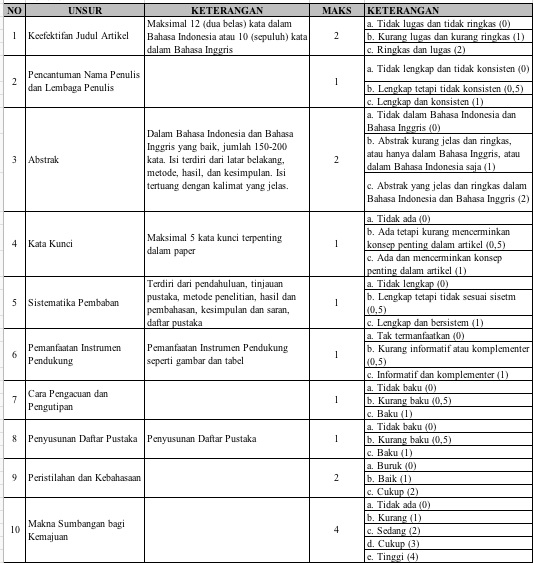
\includegraphics[width=1\textwidth]
      {figures/form1}}
      \caption{Form nilai bagian 1.}
      \label{form1}
      \end{figure}

	\begin{figure}[ht]
	      \centerline{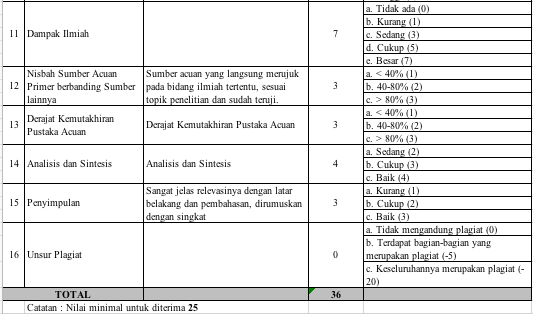
\includegraphics[width=1\textwidth]
	      {figures/form2}}
	      \caption{form nilai bagian 2.}
	      \label{form2}
	      \end{figure}

\chapter{FAQ}

M : Kalo Intership II atau TA harus buat aplikasi ?
D : Ga harus buat aplikasi tapi harus ngoding

M : Pa saya bingung mau ngapain, saya juga bingung mau presentasi apa?
D : Makanya baca de, buka jurnal topik `ganteng' nah kamu baca dulu sehari 5 kali ya, 4 hari udah 20 tuh. Bingung itu tanda kurang wawasan alias kurang baca.

M : Pa saya sudah cari jurnal terindeks scopus tapi ga nemu.
D : Kamu punya mata de? coba dicolok dulu. Kamu udah lakuin apa aja? tolong di list laporkan ke grup Tingkat Akhir. Tinggal buka google scholar klik dari tahun 2014, cek nama jurnalnya di scimagojr.com beres.

M : Pa saya belum dapat tempat intership, jadi ga tau mau presentasi apa?
D : kamu kok ga nyambung, yang dipresentasikan itu yang kamu baca bukan yang akan kamu lakukan.

M : Pa ini jurnal harus yang terindex scopus ga bisa yang lain ?
D : Index scopus menandakan artikel tersebut dalam standar semantik yang mudah dipahami dan dibaca serta bukan artikel asal jadi. Jika diluar scopus biasanya lebih sukar untuk dibaca dan dipahami karena tidak adanya proses review yang baik dan benar terhadap artikel.

M : Pa saya tidak mengerti
D : Coba lihat standar alasan

M : Pa saya bingung
D : Coba lihat standar alasan

M : Pa saya sibuk
D : Mbahmu....

M : Pa saya ganteng
D : Ndasmu....

M : Pa saya kece
D : wes karepmu lah....


Biasanya anda memiliki alasan tertentu jika menghadapi kendala saat proses bimbingan, disini saya akan melakukan standar alasan agar persepsi yang diterima sama dan tidak salah kaprah. Penggunaan kata alasan tersebut antara lain :

1. Tidak Mengerti : anda boleh menggunakan alasan ini jika anda sudah melakukan tahapan membaca dan meresumekan 15 jurnal. Sudah mencoba dan mempraktekkan teorinya dengan mencari di youtube dan google minimal 6 jam sehari selama 3 hari berturut-turut.

2. Bingung : anda boleh mengatakan alasan bingung setelah maksimal dalam berusaha menyelesaikan tugas bimbingan dari dosen(sudah dilakukan semua). Anda belum bisa mengatakan alasan bingung jika anda masih belum menyelesaikan tugas bimbingan dan poin nomor 1 diatas. Setelah anda menyelesaikan tugas bimbingan secara maksimal dan tahap 1 poin diatas, tapi anda masih tetap bingung maka anda boleh memakai alasan ini.

%next line adds the Bibliography to the contents page
\addcontentsline{toc}{chapter}{Bibliography}
%uncomment next line to change bibliography name to references
%\renewcommand{\bibname}{References}
\bibliography{references}        %use a bibtex bibliography file refs.bib
\bibliographystyle{plain}  %use the plain bibliography style

\end{document}

